\begin{figure}[htbp]
\centering
\shorthandoff{<>}
\begin{tikzpicture}[x=1.25cm,y=1cm,font=\small,>=latex]
  \foreach \x in {0,4,8}{\draw[gray!70,line width=1pt] (\x,-0.6)--(\x,3.8);}
  \draw[<->,blue!70!black] (0,-0.95)--(4,-0.95) node[midway,below] {$l$};
  \draw[<->,blue!70!black] (4,-0.95)--(8,-0.95) node[midway,below] {$l$};
  \coordinate (C) at (3.6,1.5);
  \coordinate (A) at (3.0,2.1);
  \coordinate (B) at (4.2,0.9);
  \draw[red!75!black,line width=2pt] (A)--(B);
  \fill[red!75!black] (C) circle (2pt);
  \draw[<->,orange!85!black] (3.6,2.55)--(4,2.55) node[midway,above] {$X$};
  \draw[black!65] (3.6,2.25) arc[start angle=90,end angle=45, radius=0.75];
  \node at (3.96,2.05) {$\theta$};
  \draw[dashed,black!50] (3.6,1.5)--(3.6,2.35);
  \draw[<->,teal!70!black] (3.6,1.5)--(4.2,1.5)
    node[midway,below] {$\frac{a}{2}\sin\Theta$};
  \node[anchor=west] at (4.65,3.0) {$X\sim\operatorname{Unif}(0,l/2)$};
  \node[anchor=west] at (4.65,2.35) {$\Theta\sim\operatorname{Unif}(0,\pi/2)$};
  \node[anchor=west,align=left] at (4.65,1.35) {La aguja cruza una línea\\si $X\le\dfrac{a}{2}\sin\Theta$.};
\end{tikzpicture}
\shorthandon{<>}
\caption{Geometría del problema de la aguja de Buffon. $X$ es la distancia del centro de la aguja a la línea paralela más cercana; $\Theta$ es el ángulo agudo entre la aguja y las líneas. El segmento proyectado desde el centro hasta una punta perpendicularmente a las líneas mide $(a/2)\sin\theta$.}
\label{fig:aguja-buffon}
\end{figure}